\documentclass{beamer}
\usepackage[utf8]{inputenc}

\usetheme{Madrid}
\usecolortheme{default}
\usepackage{extarrows}
\usepackage{amsmath}
\usepackage{extarrows}
\usepackage{amssymb,amsfonts,amsthm}
\usepackage{txfonts}
\usepackage{tkz-euclide}
\usepackage{listings}
\usepackage{adjustbox}
\usepackage{array}
\usepackage{tabularx}
\usepackage{gvv}
\usepackage{lmodern}
\usepackage{circuitikz}
\usepackage{tikz}
\usepackage{graphicx}
\usepackage{amsmath} 

\setbeamertemplate{page number in head/foot}[totalframenumber]

\usepackage{tcolorbox}
\tcbuselibrary{minted,breakable,xparse,skins}

\definecolor{bg}{gray}{0.95}
\DeclareTCBListing{mintedbox}{O{}m!O{}}{%
  breakable=true,
  listing engine=minted,
  listing only,
  minted language=#2,
  minted style=default,
  minted options={%
    linenos,
    gobble=0,
    breaklines=true,
    breakafter=,,
    fontsize=\small,
    numbersep=8pt,
    #1},
  boxsep=0pt,
  left skip=0pt,
  right skip=0pt,
  left=25pt,
  right=0pt,
  top=3pt,
  bottom=3pt,
  arc=5pt,
  leftrule=0pt,
  rightrule=0pt,
  bottomrule=2pt,
  toprule=2pt,
  colback=bg,
  colframe=orange!70,
  enhanced,
  overlay={%
    \begin{tcbclipinterior}
    \fill[orange!20!white] (frame.south west) rectangle ([xshift=20pt]frame.north west);
    \end{tcbclipinterior}},
  #3,
}
\lstset{
    language=C,
    basicstyle=\ttfamily\small,
    keywordstyle=\color{blue},
    stringstyle=\color{orange},
    commentstyle=\color{green!60!black},
    numbers=left,
    numberstyle=\tiny\color{gray},
    breaklines=true,
    showstringspaces=false,
}
\title %optional
{12.150}


\author 
{Kartik Lahoti - EE25BTECH11032}

\begin{document}


\frame{\titlepage}
\begin{frame}{Question}
Two sides of a triangle are represented by vectors $\vec{a} = \hat{i}+\hat{j}+\hat{k}$ and 
$\vec{b} = \hat{-i}+\hat{-j}+\hat{k}$. The area (magnitude) of the triangle is
\begin{multicols}
\begin{enumerate}
    \item $\frac{1}{\sqrt{2}}$
    \item $1$
    \item $\sqrt{2}$
    \item $2\sqrt{2}$
\end{enumerate}
\end{multicols}

\end{frame}

\begin{frame}{Theoretical Solution}
Given , 
\begin{align}
    \vec{a} = \myvec{1\\1\\1} , \quad \vec{b} = \myvec{-1\\-1\\1}
\end{align}

Area of Trianle 

\begin{align}
    \frac{1}{2}\norm{\vec{a}\times\vec{b}}
\end{align}
\end{frame}

\begin{frame}{Theoretical Solution}
Also, 

\begin{align}
    \vec{a}\times\vec{b} &= \myvec{\mydet{\vec{a}_{23} \quad \vec{b}_{23}} \\ \mydet{\vec{a}_{31} \quad \vec{b}_{31}} \\ \mydet{\vec{a}_{12} \quad \vec{b}_{12}}}
\end{align}

\begin{align}
    &= \myvec{1\cdot1 - 1\cdot\brak{-1} \\ 1\cdot\brak{-1} - 1\cdot1 \\ 1\cdot\brak{-1} - 1\cdot\brak{-1}} = \myvec{2\\-2\\0}
\end{align}
\end{frame}

\begin{frame}{Theoretical Solution}
\begin{align}
    Ar\brak{\Delta} &= \frac{1}{2}\norm{\myvec{2\\-2\\0}}\\
                    &= \frac{1}{2}2\sqrt{2}\\
                    &= \sqrt{2}
\end{align}

Hence, Answer : Option $3$
\end{frame}

\begin{frame}{Plot}
    \centering
    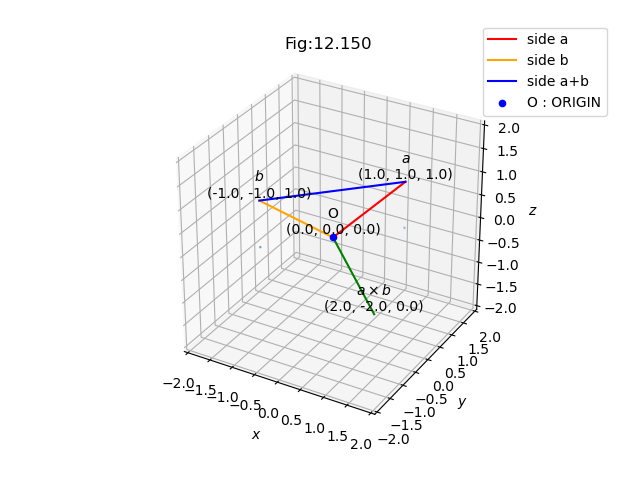
\includegraphics[width=\columnwidth, height=0.8\textheight, keepaspectratio]{../figs/vector2.png}   
\end{frame}

\end{document}
